

\tikzset{every picture/.style={line width=0.75pt}} %set default line width to 0.75pt        

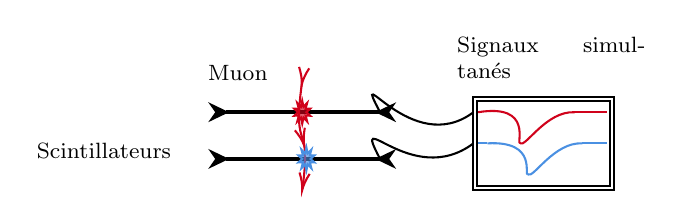
\begin{tikzpicture}[x=0.75pt,y=0.75pt,yscale=-1,xscale=1,scale=0.75]
%uncomment if require: \path (0,300); %set diagram left start at 0, and has height of 300

%Straight Lines [id:da35180804861036363] 
\draw [line width=1.5]    (201,140) -- (299,140) ;
\draw [shift={(297,140)}, rotate = 0] [fill={rgb, 255:red, 0; green, 0; blue, 0 }  ][line width=0.08]  [draw opacity=0] (13.4,-6.43) -- (0,0) -- (13.4,6.44) -- (8.9,0) -- cycle    ;
\draw [shift={(203,140)}, rotate = 180] [fill={rgb, 255:red, 0; green, 0; blue, 0 }  ][line width=0.08]  [draw opacity=0] (13.4,-6.43) -- (0,0) -- (13.4,6.44) -- (8.9,0) -- cycle    ;
%Straight Lines [id:da3704052850931778] 
\draw [line width=1.5]    (201,170) -- (299,170) ;
\draw [shift={(297,170)}, rotate = 0] [fill={rgb, 255:red, 0; green, 0; blue, 0 }  ][line width=0.08]  [draw opacity=0] (13.4,-6.43) -- (0,0) -- (13.4,6.44) -- (8.9,0) -- cycle    ;
\draw [shift={(203,170)}, rotate = 180] [fill={rgb, 255:red, 0; green, 0; blue, 0 }  ][line width=0.08]  [draw opacity=0] (13.4,-6.43) -- (0,0) -- (13.4,6.44) -- (8.9,0) -- cycle    ;
%Curve Lines [id:da5889182919658384] 
\draw [color={rgb, 255:red, 208; green, 2; blue, 27 }  ,draw opacity=1 ]   (249.7,122.17) .. controls (243.47,168.16) and (256.24,144.2) .. (250.19,188.63) ;
\draw [shift={(250,190)}, rotate = 277.99] [color={rgb, 255:red, 208; green, 2; blue, 27 }  ,draw opacity=1 ][line width=0.75]    (10.93,-3.29) .. controls (6.95,-1.4) and (3.31,-0.3) .. (0,0) .. controls (3.31,0.3) and (6.95,1.4) .. (10.93,3.29)   ;
\draw [shift={(251.28,161.38)}, rotate = 255.17] [color={rgb, 255:red, 208; green, 2; blue, 27 }  ,draw opacity=1 ][line width=0.75]    (10.93,-3.29) .. controls (6.95,-1.4) and (3.31,-0.3) .. (0,0) .. controls (3.31,0.3) and (6.95,1.4) .. (10.93,3.29)   ;
\draw [shift={(249.7,122.17)}, rotate = 278.07] [color={rgb, 255:red, 208; green, 2; blue, 27 }  ,draw opacity=1 ][line width=0.75]    (10.93,-3.29) .. controls (6.95,-1.4) and (3.31,-0.3) .. (0,0) .. controls (3.31,0.3) and (6.95,1.4) .. (10.93,3.29)   ;
%Curve Lines [id:da7185776494259334] 
\draw    (300,140) .. controls (280.6,103) and (320,170) .. (360,140) ;
%Curve Lines [id:da14145211725039786] 
\draw    (300,170) .. controls (280.6,133) and (320,190) .. (360,160) ;
%Shape: Frame [id:dp6591001505040031] 
\draw   (360,130) -- (450,130) -- (450,190) -- (360,190) -- cycle(447.45,132.55) -- (362.55,132.55) -- (362.55,187.45) -- (447.45,187.45) -- cycle ;
%Curve Lines [id:da8731678176500584] 
\draw [color={rgb, 255:red, 208; green, 2; blue, 27 }  ,draw opacity=1 ]   (363,140) .. controls (399,134.2) and (387,161.4) .. (390,160) ;
%Curve Lines [id:da7130259646710352] 
\draw [color={rgb, 255:red, 208; green, 2; blue, 27 }  ,draw opacity=1 ]   (425,140) .. controls (406.8,139) and (393.2,163) .. (390,160) ;
%Curve Lines [id:da9843154919629533] 
\draw [color={rgb, 255:red, 74; green, 144; blue, 226 }  ,draw opacity=1 ]   (369,160) .. controls (401.8,158.2) and (392,181.4) .. (395,180) ;
%Curve Lines [id:da24171517075659743] 
\draw [color={rgb, 255:red, 74; green, 144; blue, 226 }  ,draw opacity=1 ]   (430,160) .. controls (411.8,159) and (398.2,183) .. (395,180) ;
%Straight Lines [id:da35050420120468406] 
\draw [color={rgb, 255:red, 74; green, 144; blue, 226 }  ,draw opacity=1 ]   (430,160) -- (446,160) ;
%Straight Lines [id:da2379289101719989] 
\draw [color={rgb, 255:red, 208; green, 2; blue, 27 }  ,draw opacity=1 ]   (424,140) -- (446,140) ;
%Straight Lines [id:da8809434112734575] 
\draw [color={rgb, 255:red, 74; green, 144; blue, 226 }  ,draw opacity=1 ]   (363,160) -- (369,160) ;
%Shape: Star [id:dp0028643894481888976] 
\draw  [color={rgb, 255:red, 208; green, 2; blue, 27 }  ,draw opacity=1 ][fill={rgb, 255:red, 208; green, 2; blue, 27 }  ,fill opacity=0.63 ] (250,132.68) -- (250.83,136.52) -- (253.16,134.08) -- (252.17,137.85) -- (255.11,137.74) -- (252.69,140) -- (255.11,142.26) -- (252.17,142.15) -- (253.16,145.92) -- (250.83,143.48) -- (250,147.32) -- (249.17,143.48) -- (246.84,145.92) -- (247.83,142.15) -- (244.89,142.26) -- (247.31,140) -- (244.89,137.74) -- (247.83,137.85) -- (246.84,134.08) -- (249.17,136.52) -- cycle ;
%Shape: Star [id:dp4313697147068123] 
\draw  [color={rgb, 255:red, 74; green, 144; blue, 226 }  ,draw opacity=1 ][fill={rgb, 255:red, 74; green, 144; blue, 226 }  ,fill opacity=0.61 ] (252.69,162.68) -- (253.52,166.52) -- (255.85,164.08) -- (254.86,167.85) -- (257.8,167.74) -- (255.38,170) -- (257.8,172.26) -- (254.86,172.15) -- (255.85,175.92) -- (253.52,173.48) -- (252.69,177.32) -- (251.86,173.48) -- (249.53,175.92) -- (250.51,172.15) -- (247.58,172.26) -- (250,170) -- (247.58,167.74) -- (250.51,167.85) -- (249.53,164.08) -- (251.86,166.52) -- cycle ;

% Text Node
\draw (140,165) node   [align=left] {\begin{minipage}[lt]{68pt}\setlength\topsep{0pt}
\footnotesize{Scintillateurs}
\end{minipage}};
% Text Node
\draw (250,115) node   [align=left] {\begin{minipage}[lt]{68pt}\setlength\topsep{0pt}
\footnotesize{Muon}
\end{minipage}};
% Text Node
\draw (410,105) node   [align=left] {\begin{minipage}[lt]{68pt}\setlength\topsep{0pt}
\footnotesize{Signaux simultanés}
\end{minipage}};


\end{tikzpicture}
